\documentclass[12pt]{article}
\usepackage{graphicx}
\usepackage{caption}

\linespread{1.25}

\title{Processing of Scalar Implicatures and Question Under Discussion} 

% \author{}
% \date{}

\begin{document} 

\maketitle 

\section{Methods}

\subsection*{Participants}

Participants (US IP Addresses, prior approval rating > 95\%) were recruited on Amazon Mechanical Turk and were paid \$2.3.

\begin{table}[h]
\begin{tabular}{ccccccc}
& \multicolumn{3}{c}{Before Exclusions} & \multicolumn{3}{c}{After Exclusions} \\
& all QUD & any QUD & no QUD & all QUD & any QUD & no QUD \\
Experiment 1 & 50 & 50 & 50 & 41 & 35 & 38 \\
Experiment 2 & 50 & 50 & 50 & 37 & 36 & 38 \\
Experiment 3 & 200 & 200 & 200 & fill & fill & fill \\
Experiment 4 & 400 & 400 & 400 & 281 & 256 & 313
\end{tabular}
\end{table}

\subsection*{Procedure and Materials}

At the beginning of the experiment, participants in each group were presented with a different cover story. These cover stories were designed to establish an implicit QUD.
\paragraph{all QUD} Participants in all QUD group read a story explaining them that they are at a candy store and testing a row of special gumball machines. These gumball machines have 13 gumballs in their upper chambers and when they distribute gumballs, you see a certain number of gumballs move to the lower chamber. These machines also say how many gumballs you got (“You got X gumballs”), but are sometimes faulty in their report. The store worker’s boss has threatened to fire him if the gumball machines are left empty and he cannot see the machines from the register and only tell how full they are by their statements. Participants were asked to help the store worker by telling him if this statement is right or wrong by pressing the yes or no key.

\begin{center}Is the machine empty? $\rightarrow$ Did I get all of the gumballs?\end{center}

\paragraph{any QUD} In the any QUD group, participants read the same story except, in their story, the store worker’s boss has threatened to fire him if the gumball machines get jammed. 

\begin{center}Is the machine jammed? $\rightarrow$ Did I get none of the gumballs?\end{center}

\paragraph{no QUD} Participants in no QUD group didn’t read a cover story but instead read instructions that explained that they were going to see a gumball machine filled with gumballs and after a few seconds certain number of gumballs will move to its bottom chamber and the machine will say how many gumballs you got. Participants were asked to say if this statement right or wrong by pressing the yes or no key.

\begin{center}Is the statement correct? $\rightarrow$ No implicit QUD\end{center}

\paragraph{}After reading the cover story, participants went through a scripted demonstration that showed various scenarios and the store worker’s reaction to their responses. In the all QUD condition, when all of gumballs dropped from the upper chamber to the lower chamber and the machine reported “You got all of the gumballs”, participants were asked to press the yes key and they read that they let the store worker know that the machine is empty and he therefore knows that he needs to refill the machine. They also read that one time someone got all of the gumballs and was told “You got all of the gumballs”, they pressed the no key and the store worker was fired because he didn’t refill the machine. In the any QUD condition, participants got no gumballs and the machine reported “You got none of the gumballs”. Participants were asked to press the yes key and read that they let the store worker know that the machine is not distributing gumballs and that he needs to fix the machine. They read that one time someone got 0 gumballs and was told “You got none of the gumballs”, they pressed the no key and the store worker was fired because he didn’t repair the machine. In the no QUD condition, the only feedback that participants got was a sentence that said whether they agreed or disagreed with the statement.

\paragraph{}To ensure that participants paid attention to the cover story, participants in all QUD and any QUD conditions were asked a multiple-choice question about when the store worker will be fired. For the all QUD group the correct answer was “when the machines are empty” and for the any QUD group the correct answer was “when the machines jam”. When participants answered this question incorrectly they were presented with the cover story again and went through the demonstration. Halfway through the experiment, participants were asked to answer this multiple-choice question again. This time, when they answered incorrectly they were only asked to try again. This was done to prevent the decay of the implicit QUD over time. 

\paragraph{}There were 4 practice trials with “You got all of the gumballs” and “You got none of the gumballs” statements. On 2 of these trials, the statement was correct, and on 2 of them it was incorrect. 

\paragraph{}After the practice trials, there were 72 experimental trials. The number of gumballs in the lower chamber (0 to 13 gumballs) and the quantifier in the statement (some, none, all) were varied.  On 32 of the trials the expected answer was yes, and on 32 of the trials the expected answer was no. The remaining 8 trials were occurrences of the critical trial and the main focus of this experiment. On these trials, all thirteen of the gumballs dropped to the lower chamber and participants hear the statement “You got some of the gumballs”. This statement is true when it’s interpreted semantically as “You got some and possibly all of the gumballs” but when it’s interpreted pragmatically as “You got some but not all of the gumballs”, it’s false.

\begin{center}INSERT TABLE HERE - STIMULI LIST\end{center}

Experiments differed from each other in the following ways:\\
\textbf{Experiment 1.} In the critical condition, participants heard "You got some gumballs".\\
\textbf{Experiment 2.} In the critical condition, participants heard "You got some of the gumballs".\\
\textbf{Experiment 3.} Participants were prescreened for age. Only participants aged between 18 and 25 and participants older than 45 were recruited.\\
\textbf{Experiment 4.} Participants had 4 seconds to respond after they heard the statement. 

*Both in Experiment 3 and 4 participants heard "You got some of the gumballs" in the critical condition.

\section{Results}

\paragraph{Exclusions}
The exclusion criteria and the number of participants excluded with each criterion are given below:

\begin{enumerate}
\item non-native English speakers 
\item participants who get at least two practice trials wrong 
\item participants who get the audio check wrong more than one once 
\item participants who get the second comprehension question wrong more than twice 
\item participants with accuracy of lower than 85\% on non-critical trials 
\item response times that are 2.5 standard deviations above the mean for that condition or that are faster than the onset of the quantifier.
\end{enumerate}

\begin{table}[h]
    \begin{tabular}{ccccc}
     & experiment 1 & experiment 2  & experiment 3*  & experiment 4 \\
    1 & 0 & 3 & 13 & 37 \\
    2 & 32 & 24 & 23** & 93** \\
    3 & 0 & 0 & 1 & 5 \\
    4 & 0 & 1 & 0 & 15 \\
    5 & 4 & 7 & 26 & 200*** \\
    \textbf{total} & \textbf{36} & \textbf{35} & \textbf{62} & \textbf{350} \\
    \end{tabular}
\end{table}

    *7 participants were excluded because their age didn't match the age they reported in prescreening. \\ 
    ***Criterion was changed to only exlude participants who got more than two practice trials wrong. \\
    ***Criterion was changed to only exclude participants with accuracy lower than 85\% on non-critical trials with quantifiers "some", "all", "none", and numbers below 6.

    \subsection*{Judgements}

In all four experiments, in the critical condition, participants in the all QUD group gave more pragmatic responses than the participants in the any QUD group and participants in the any QUD group gave more pragmatic responses than the no QUD group.  
\\
\begin{figure}[!h]  
    \begin{minipage}{.5\textwidth}
        \caption*{Experiment 1}
        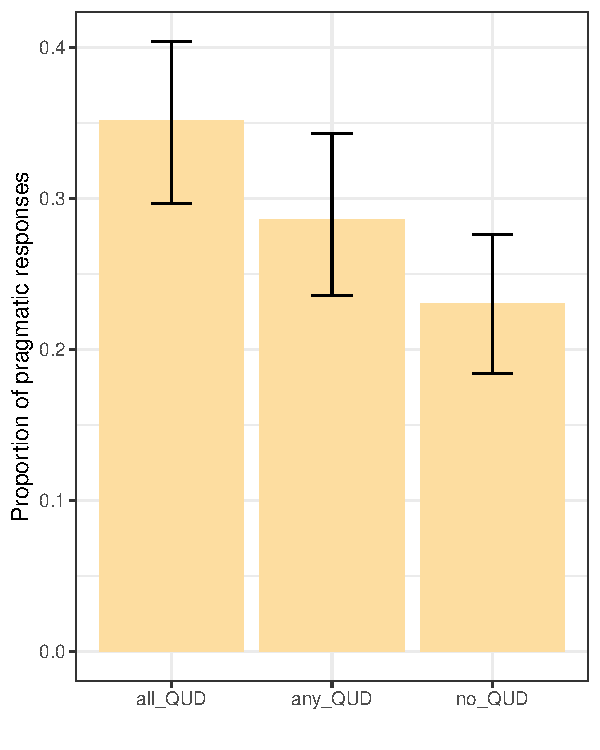
\includegraphics[height=6cm]{img/exp1_proportion_pragmatic.pdf}
    \end{minipage}%
    \begin{minipage}{.5\textwidth}
        \caption*{Experiment 2}
        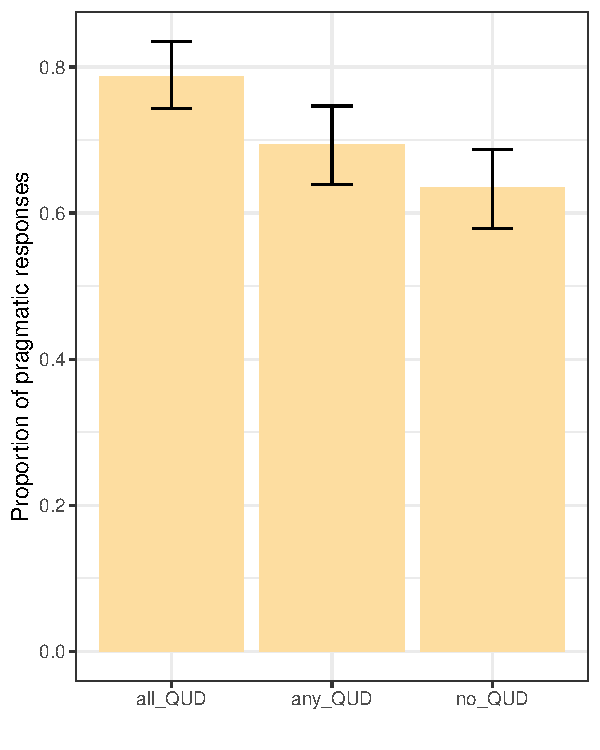
\includegraphics[height=6cm]{img/exp2_proportion_pragmatic.pdf}    
    \end{minipage}%
    \\
    \begin{minipage}{.5\textwidth}
        \caption*{Experiment 3}
        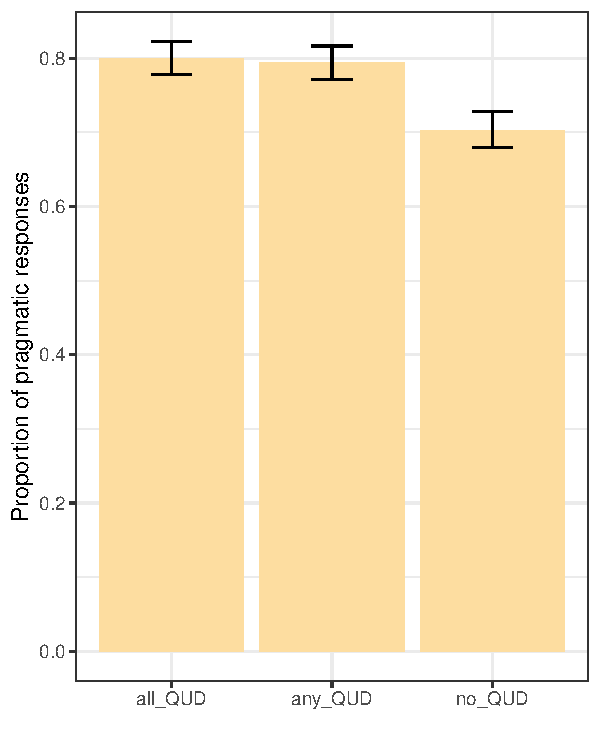
\includegraphics[height=6cm]{img/exp3_proportion_pragmatic.pdf}    
    \end{minipage}%
    \begin{minipage}{.5\textwidth}
        \caption*{Experiment 4}
        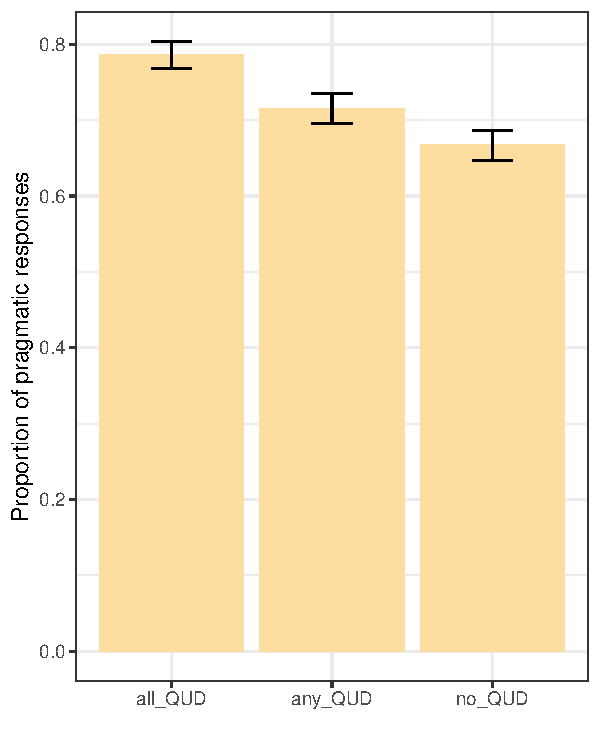
\includegraphics[height=6cm]{img/exp4_proportion_pragmatic.pdf}
    \end{minipage}%
    \caption{Proportion of pragmatic responses on critical trials for all four experiments}
\end{figure}

cover story $\rightarrow$ implicit QUD $\rightarrow$ likelihood of pragmatic responses $\rightarrow$ scaler implicature

\begin{figure}[!h] 
    \centering
    \begin{minipage}{.5\textwidth}
    \caption*{Experiment 1}
    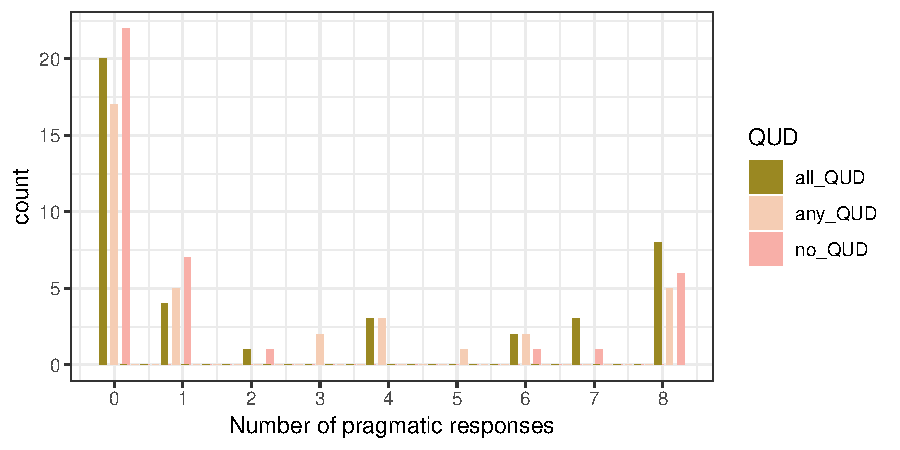
\includegraphics[height=4cm]{img/exp1_count_pragmatic.pdf}
    \end{minipage}%
    \begin{minipage}{.5\textwidth}
    \caption*{Experiment 2}
    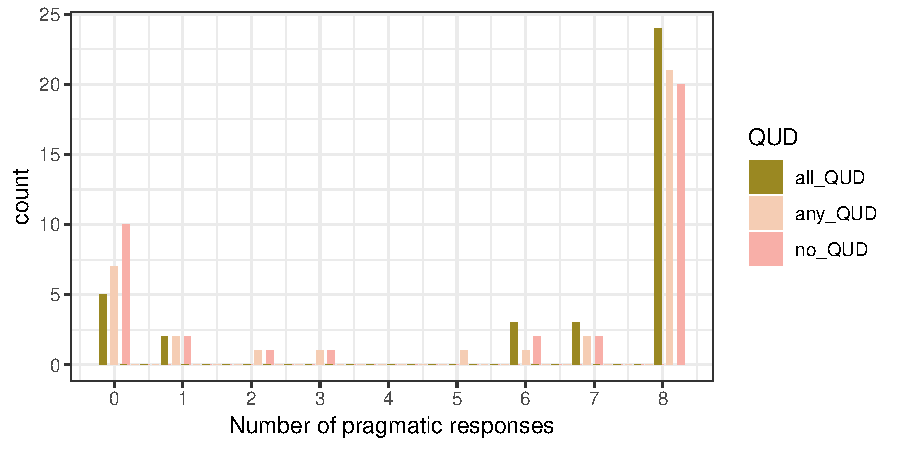
\includegraphics[height=4cm]{img/exp2_count_pragmatic.pdf}
    \end{minipage}%
    \\
    \begin{minipage}{.5\textwidth}
    \caption*{Experiment 3}
    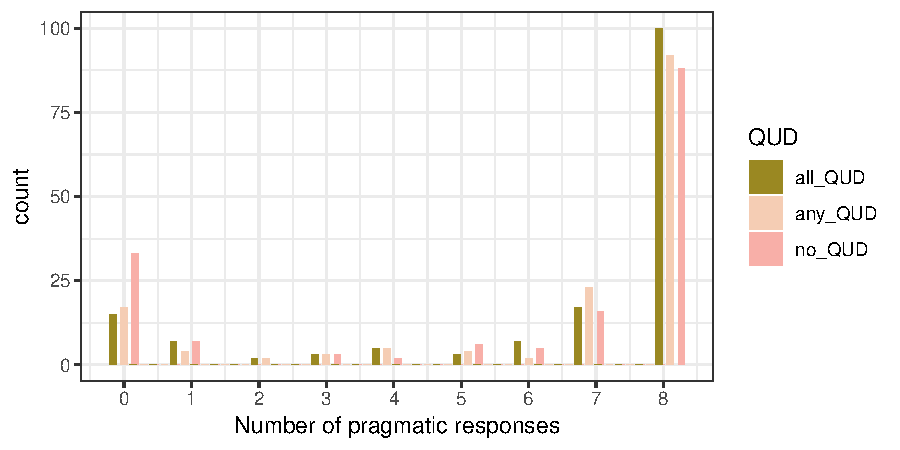
\includegraphics[height=4cm]{img/exp3_count_pragmatic.pdf}
    \end{minipage}%
    \begin{minipage}{.5\textwidth}
    \caption*{Experiment 4}
    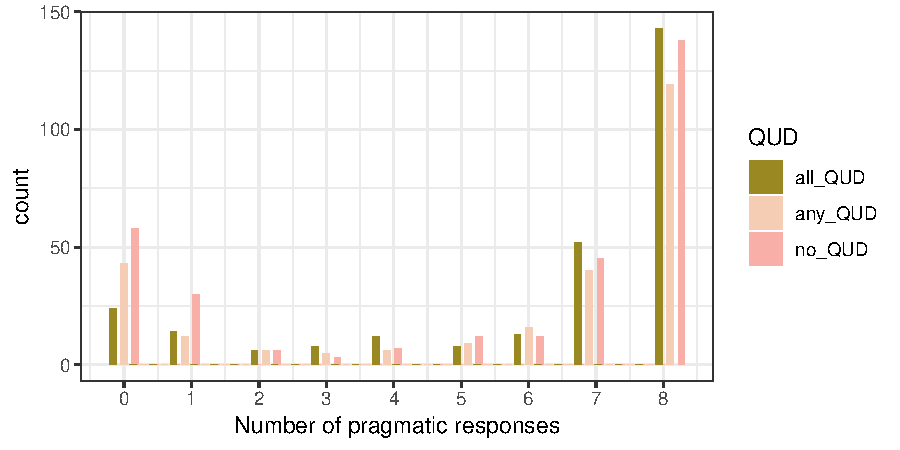
\includegraphics[height=4cm]{img/exp4_count_pragmatic.pdf}
    \end{minipage}%
    \caption{Distribution of participants over number of pragmatic responses on critical trials}
\end{figure}

\pagebreak
\subsection*{Response Times}

\begin{figure}[!h] 
    \centering
    \begin{minipage}{.5\textwidth}
        \caption*{Experiment 1}
        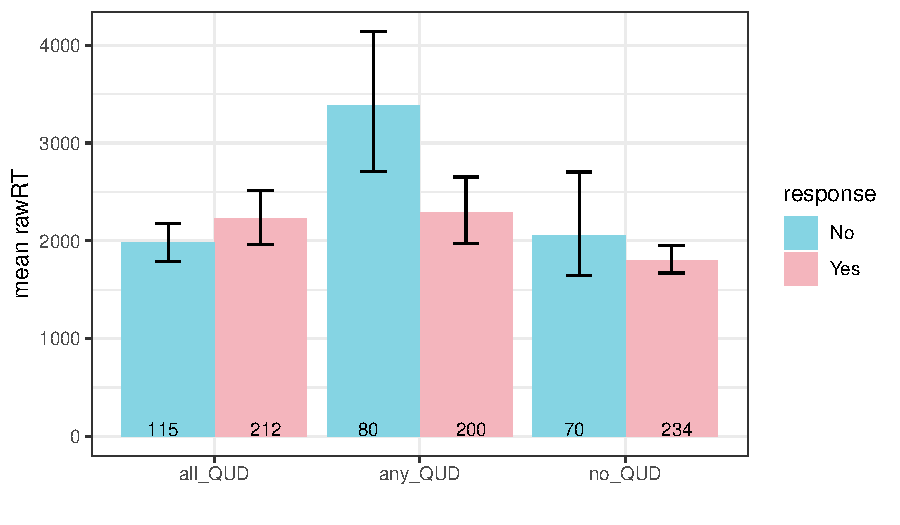
\includegraphics[height=4cm]{img/exp1_response_time.pdf}
    \end{minipage}%
    \begin{minipage}{.5\textwidth}
        \caption*{Experiment 2}
        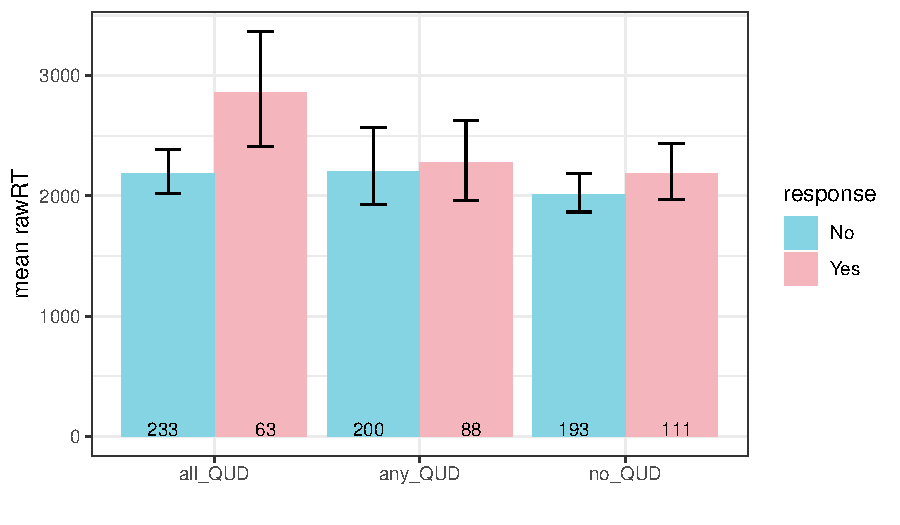
\includegraphics[height=4cm]{img/exp2_response_time.pdf}
    \end{minipage}%
    \\
    \begin{minipage}{.5\textwidth}
        \caption*{Experiment 3}
        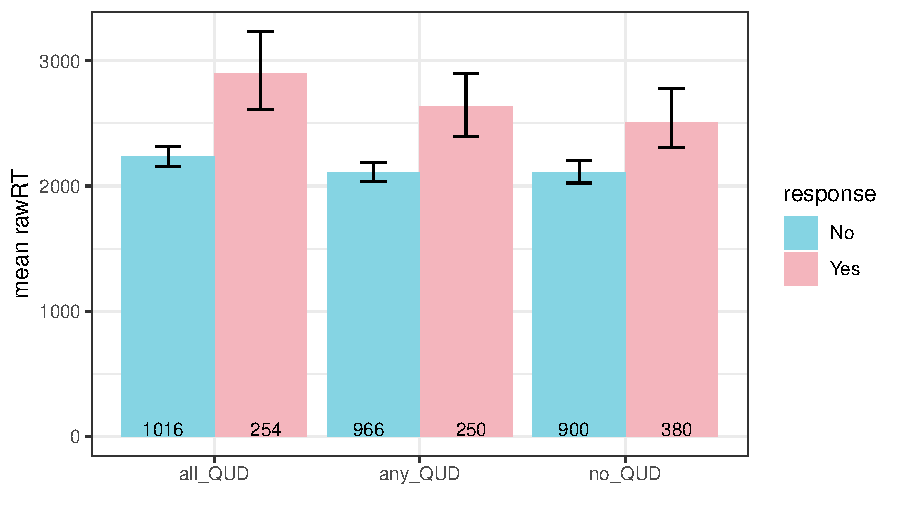
\includegraphics[height=4cm]{img/exp3_response_time.pdf}
    \end{minipage}%
    \begin{minipage}{.5\textwidth}
        \caption*{Experiment 4}
        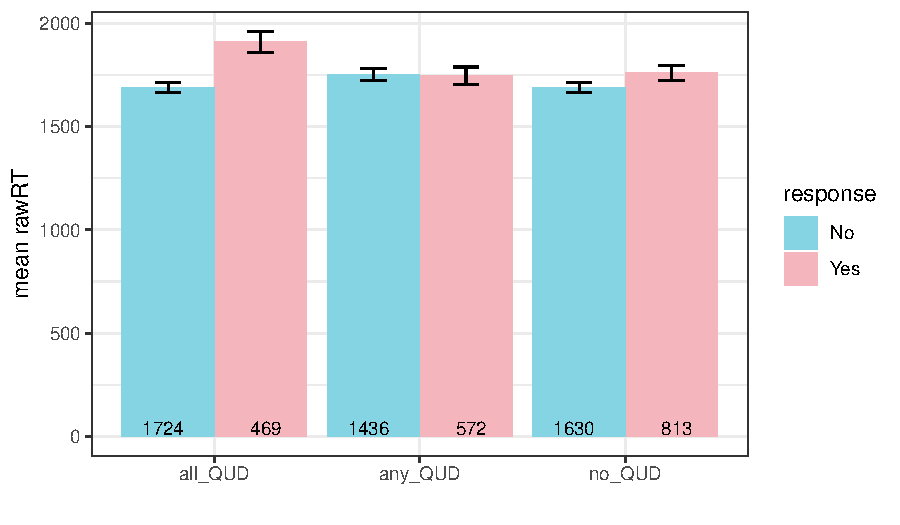
\includegraphics[height=4cm]{img/exp4_response_time.pdf}
    \end{minipage}%
    \caption{Mean response times for semantic and pragmatic responses on critical trials as a function of QUD}
\end{figure}

\pagebreak
\subsubsection*{For semantic and pragmatic responders}
\begin{figure}[!h] 
    \centering
    \begin{minipage}{.5\textwidth}
        \caption*{Experiment 1}
        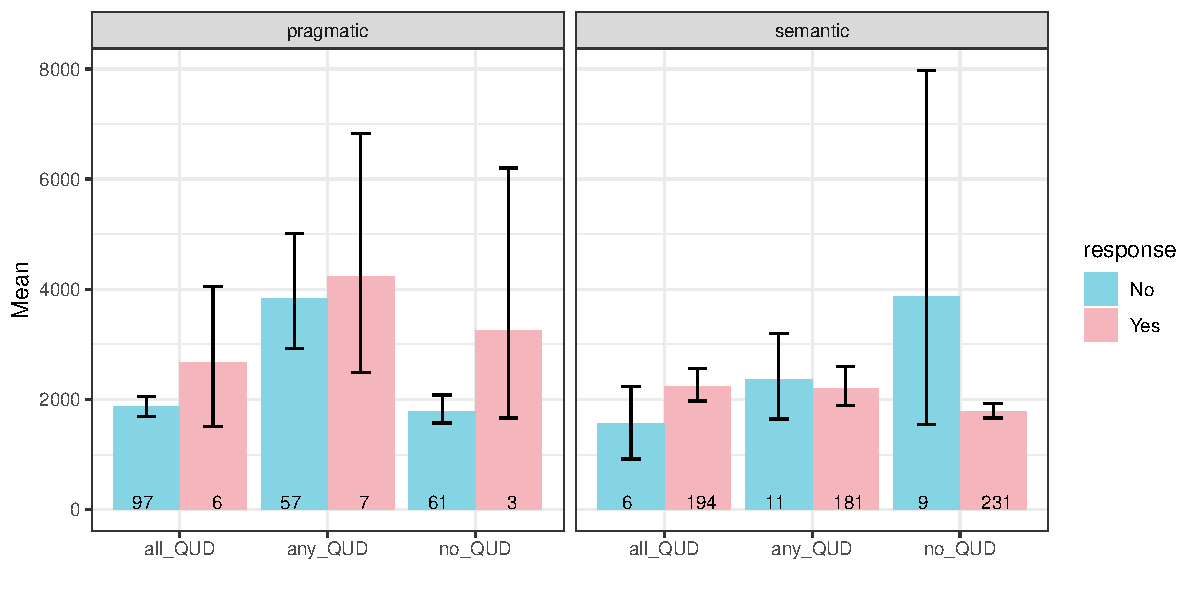
\includegraphics[height=3.5cm]{img/exp1_responder.pdf}
    \end{minipage}%
    \begin{minipage}{.5\textwidth}
        \caption*{Experiment 2}
        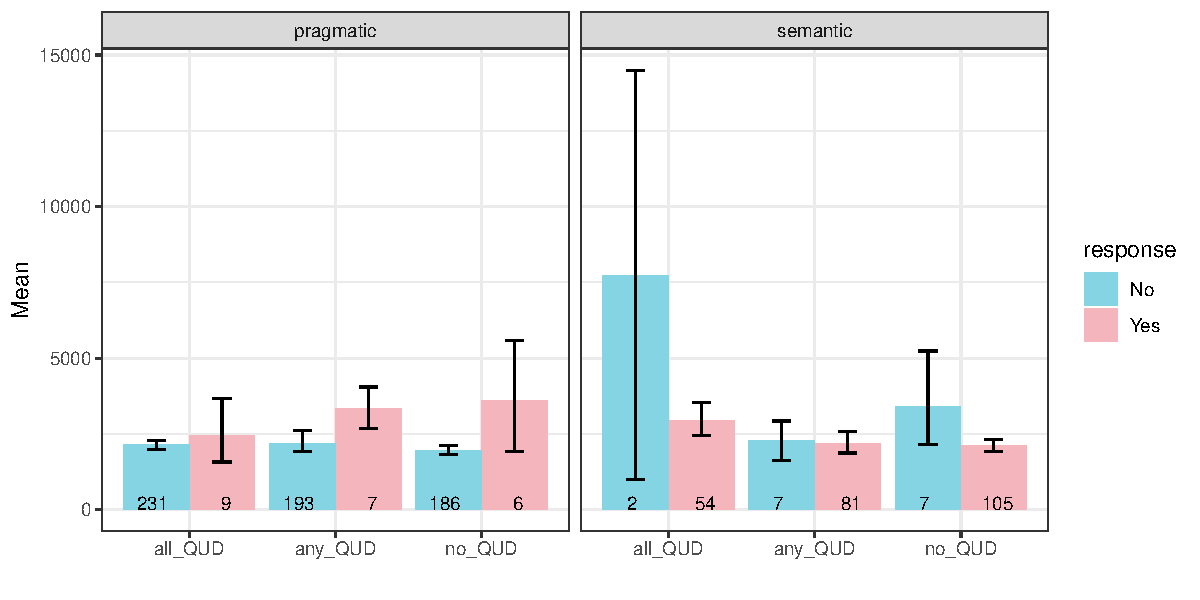
\includegraphics[height=3.5cm]{img/exp2_responder.pdf}
    \end{minipage}%
    \\
    \begin{minipage}{.5\textwidth}
        \caption*{Experiment 3}
        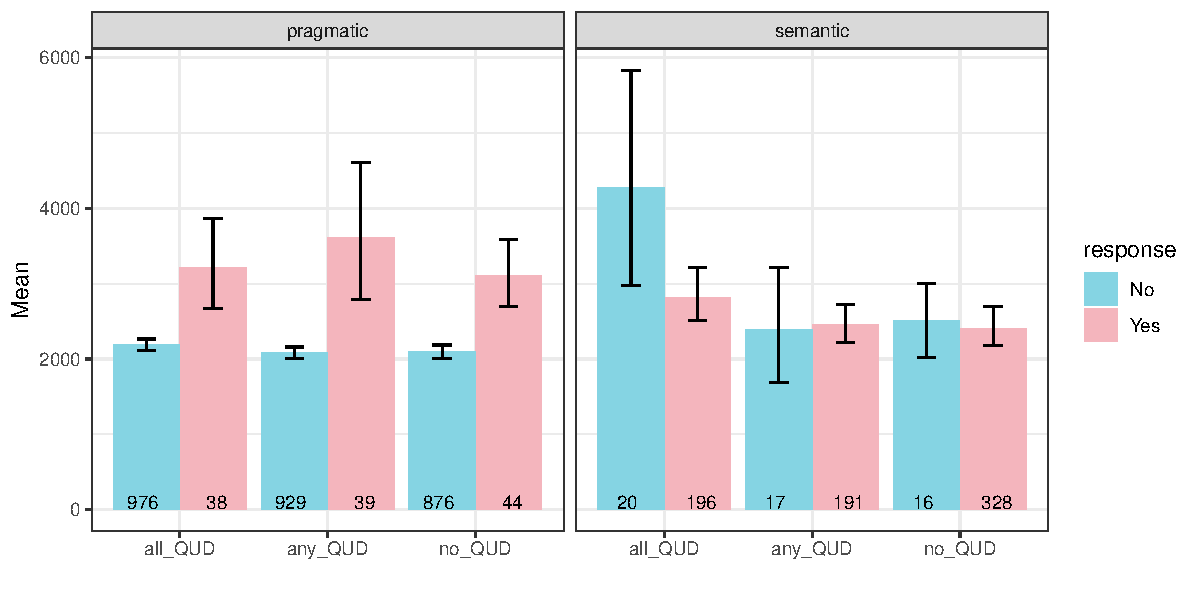
\includegraphics[height=3.5cm]{img/exp3_responder.pdf}
    \end{minipage}%
    \begin{minipage}{.5\textwidth}
        \caption*{Experiment 4}
        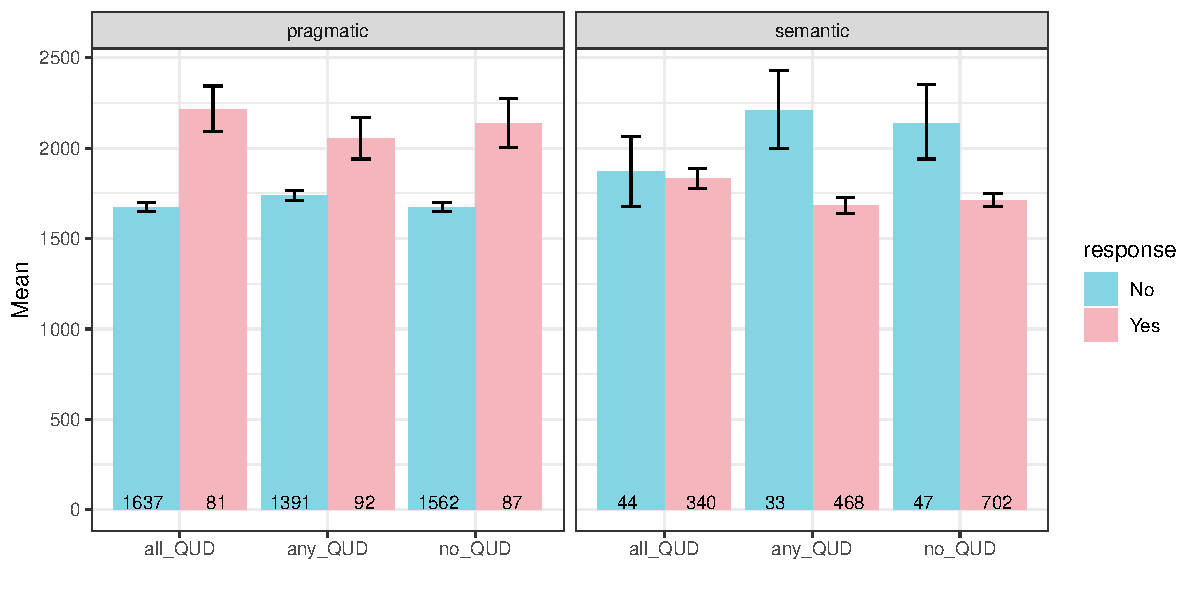
\includegraphics[height=3.5cm]{img/exp4_responder.pdf}
    \end{minipage}%
    \caption{Mean response times for semantic and pragmatic responders (inconsistent responders excluded)}
\end{figure}

\pagebreak
\subsection*{Age Effect}
\subsubsection*{Age, response type, QUD}
\begin{figure}[!h] 
    \centering
    \begin{minipage}{.5\textwidth}
        \caption*{Experiment 1}
        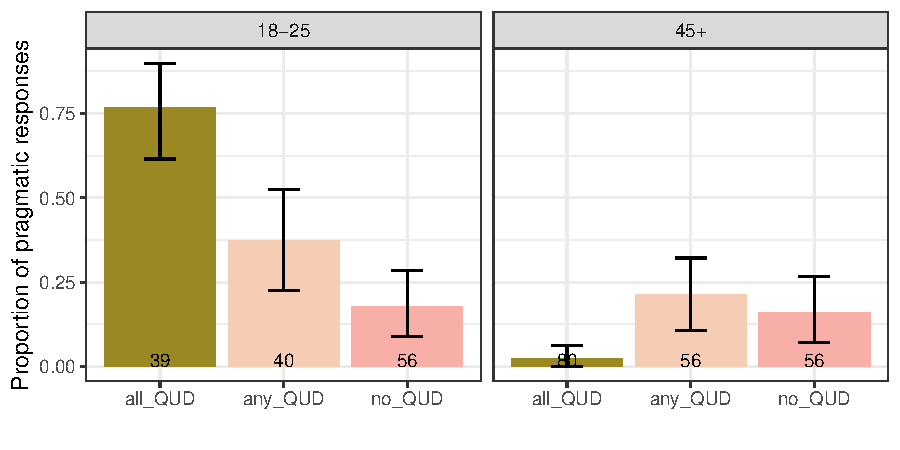
\includegraphics[height=3cm]{img/exp1_age_pragmatic.pdf}
    \end{minipage}%
    \begin{minipage}{.5\textwidth}
        \caption*{Experiment 2}
        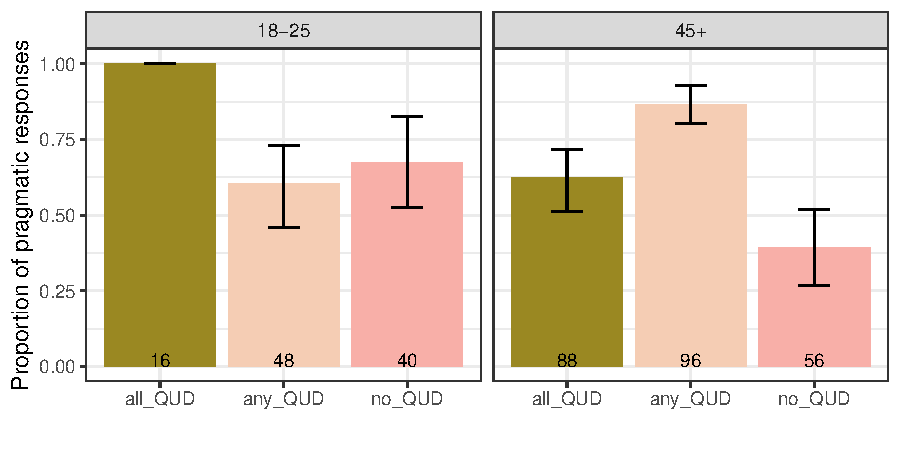
\includegraphics[height=3cm]{img/exp2_age_pragmatic.pdf}
    \end{minipage}%
    \\
    \begin{minipage}{.5\textwidth}
        \caption*{Experiment 3}
        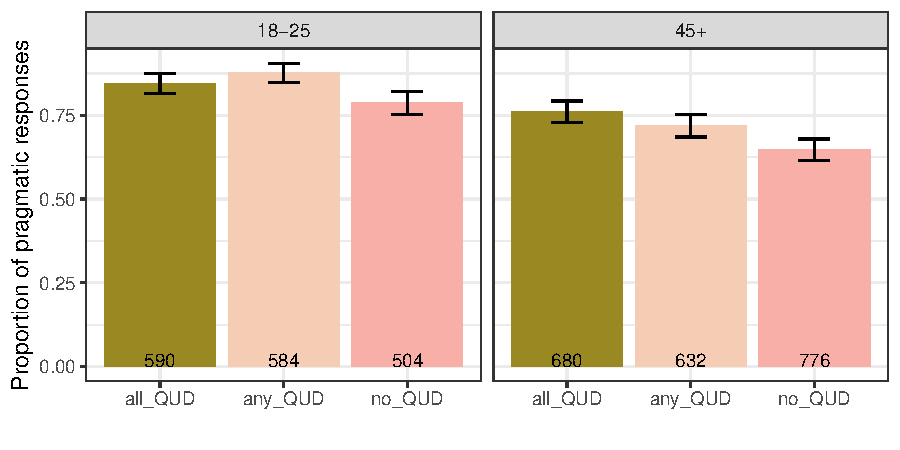
\includegraphics[height=3cm]{img/exp3_age_pragmatic.pdf}
    \end{minipage}%
    \begin{minipage}{.5\textwidth}
        \caption*{Experiment 4}
        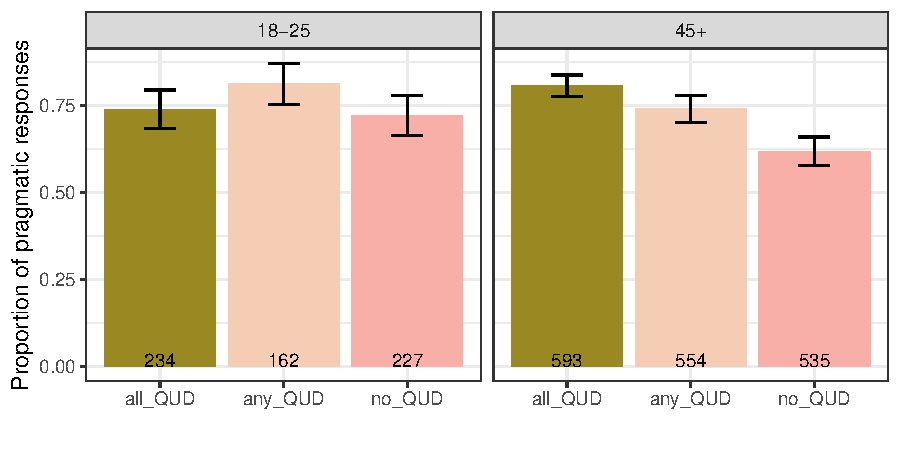
\includegraphics[height=3cm]{img/exp4_age_pragmatic.pdf}
    \end{minipage}%
    \caption{Proportion of pragmatic responses as a function of age and QUD}
\end{figure}

\pagebreak
\subsubsection*{Age, response time, QUD}
\begin{figure}[!h] 
    \centering
    \begin{minipage}{.5\textwidth}
        \caption*{Experiment 1}
        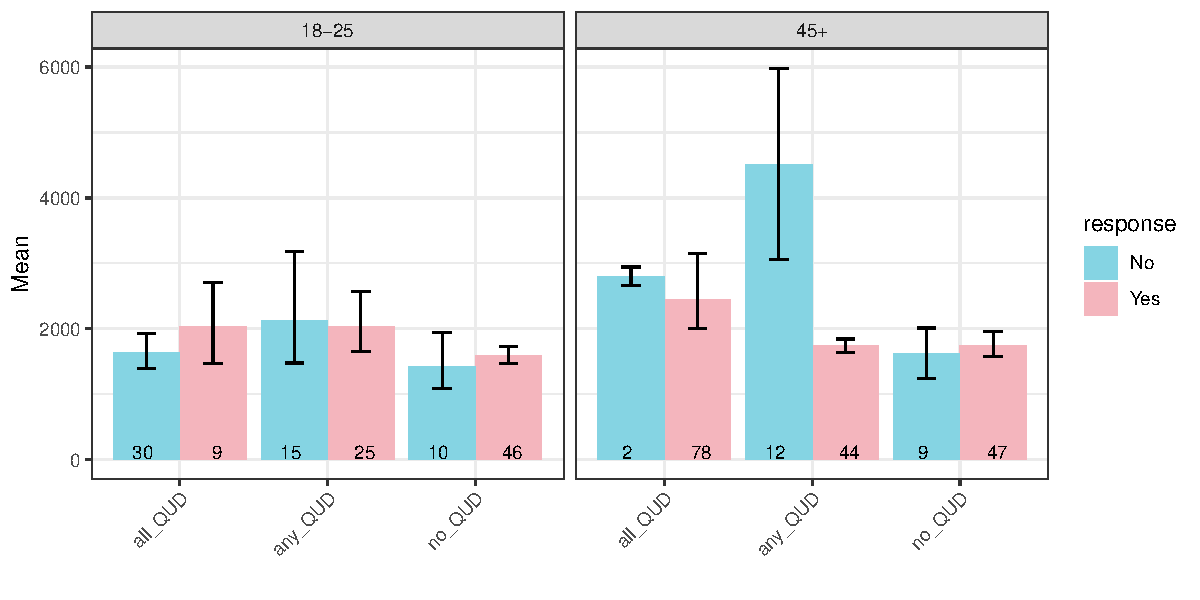
\includegraphics[height=3cm]{img/exp1_age_time.pdf}
    \end{minipage}%
    \begin{minipage}{.5\textwidth}
        \caption*{Experiment 2}
        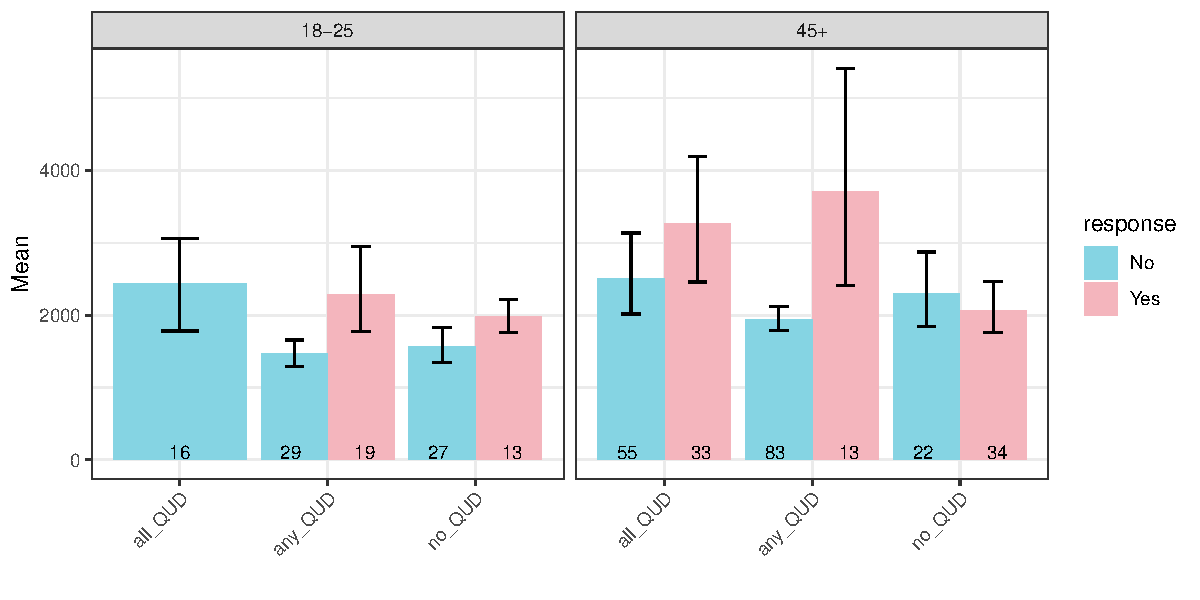
\includegraphics[height=3cm]{img/exp2_age_time.pdf}
    \end{minipage}%
    \\
    \begin{minipage}{.5\textwidth}
        \caption*{Experiment 3}
        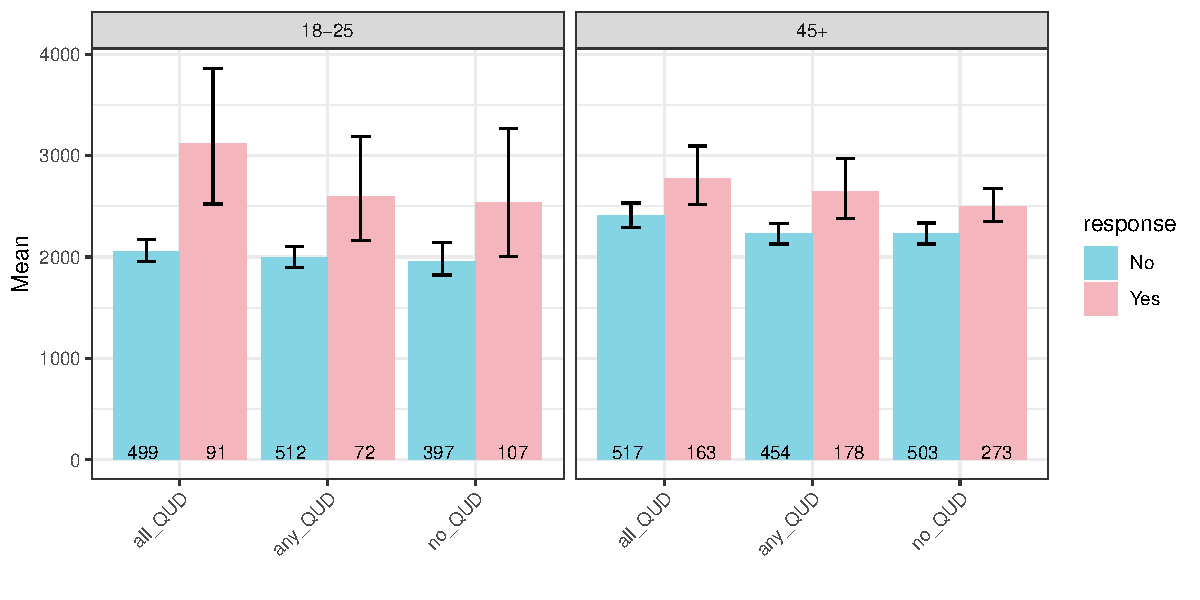
\includegraphics[height=3cm]{img/exp3_age_time.pdf}
    \end{minipage}%
    \begin{minipage}{.5\textwidth}
        \caption*{Experiment 4}
        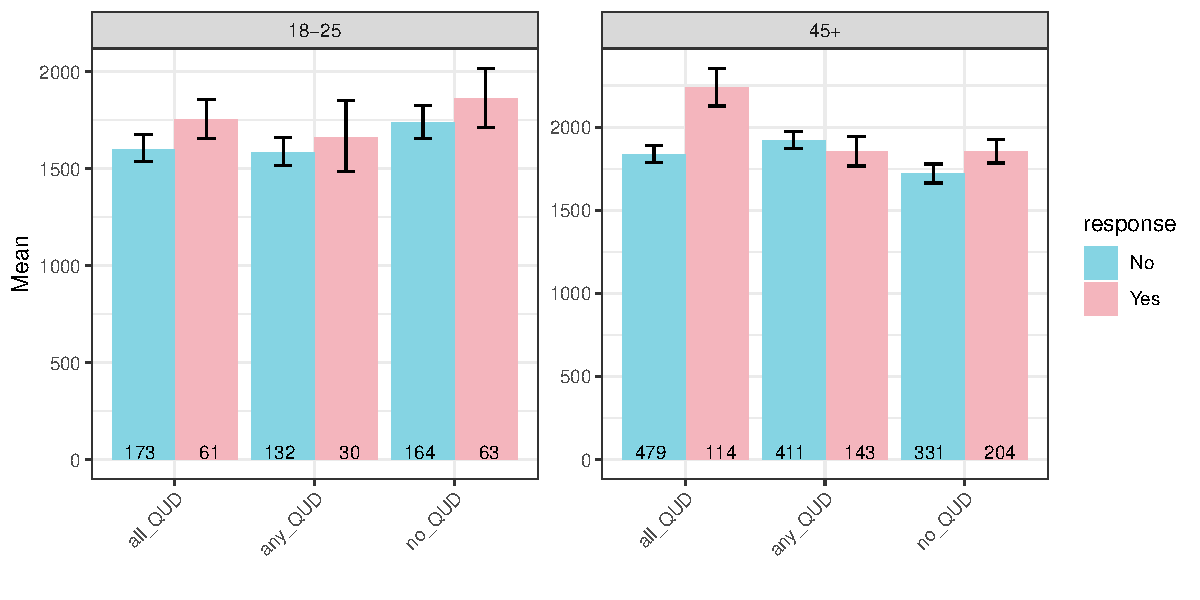
\includegraphics[height=3cm]{img/exp4_age_time.pdf}
    \end{minipage}%
    \caption{Mean response times for semantic and pragmatic responses as a function of age and QUD}
\end{figure}

\pagebreak
NOT SURE ABOUT THESE GRAPHS?
\subsubsection*{Age, responder type, response type, QUD}
\subsubsection*{Age, responder type, response time, QUD}
\pagebreak

\section*{Models - for experiment 4 (time pressure)}
\begin{enumerate}    
\item Mixed effects logistic regression predicting response type with random by-participant intercepts, from fixed effects of QUD
\\
\textbf{Prediction:} Main effect of QUD such that there are more pragmatic responses for all-QUD compared to any-QUD and no-QUD
\\ \\
% \caption*{Model1}
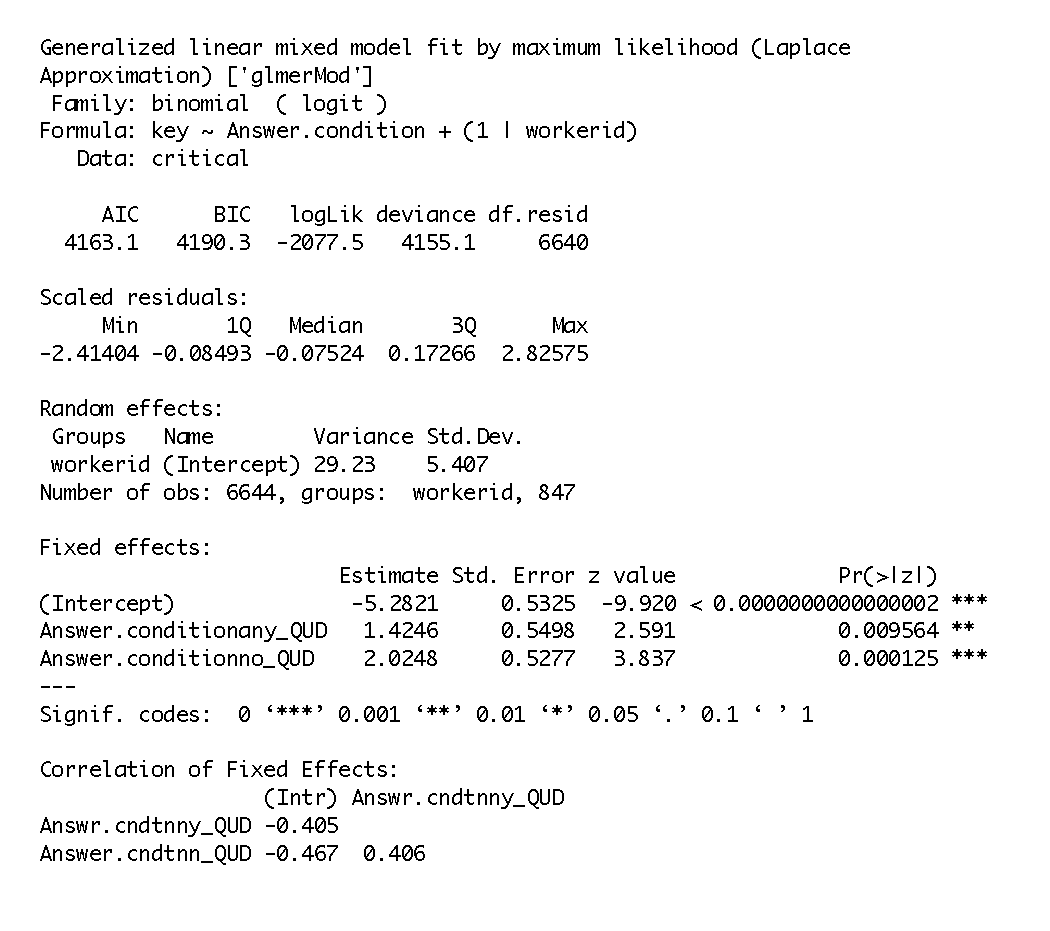
\includegraphics[height=10cm]{models/exp4_model1.pdf}
\pagebreak
\item Mixed effects linear regression model with random by-participant intercepts predicting log-transformed response time from fixed effects of QUD, response type and their interaction
\\
\textbf{Prediction:} Interaction of QUD and response such that the more relevant the alternative, the faster the pragmatic responses become and the slower the semantic responses become
\\ \\
% \caption*{Model2}
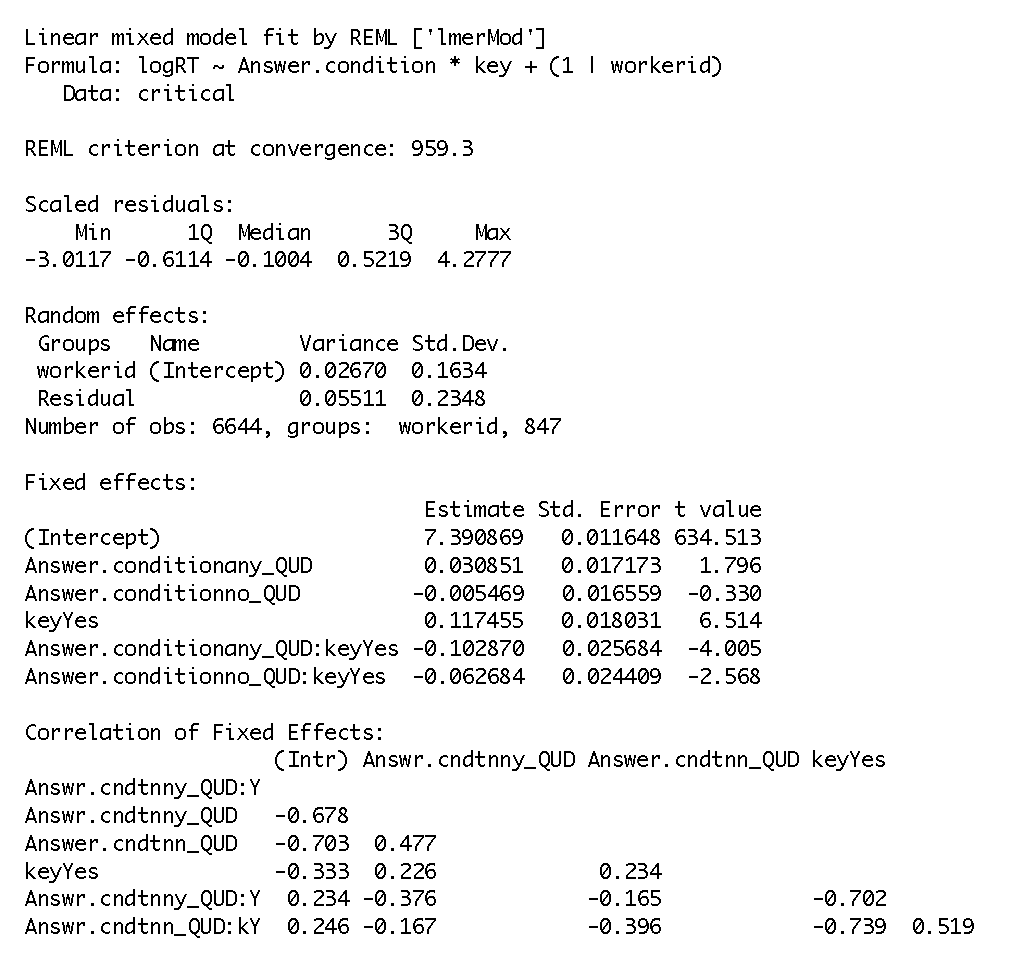
\includegraphics[height=10cm]{models/exp4_model2.pdf}
\pagebreak
\item Mixed effects logistic regression predicting response type with random by-participant intercepts, from fixed effects of QUD, responder type and their interaction
\\
\textbf{Prediction:} Prediction
% \caption*{Model3}
% 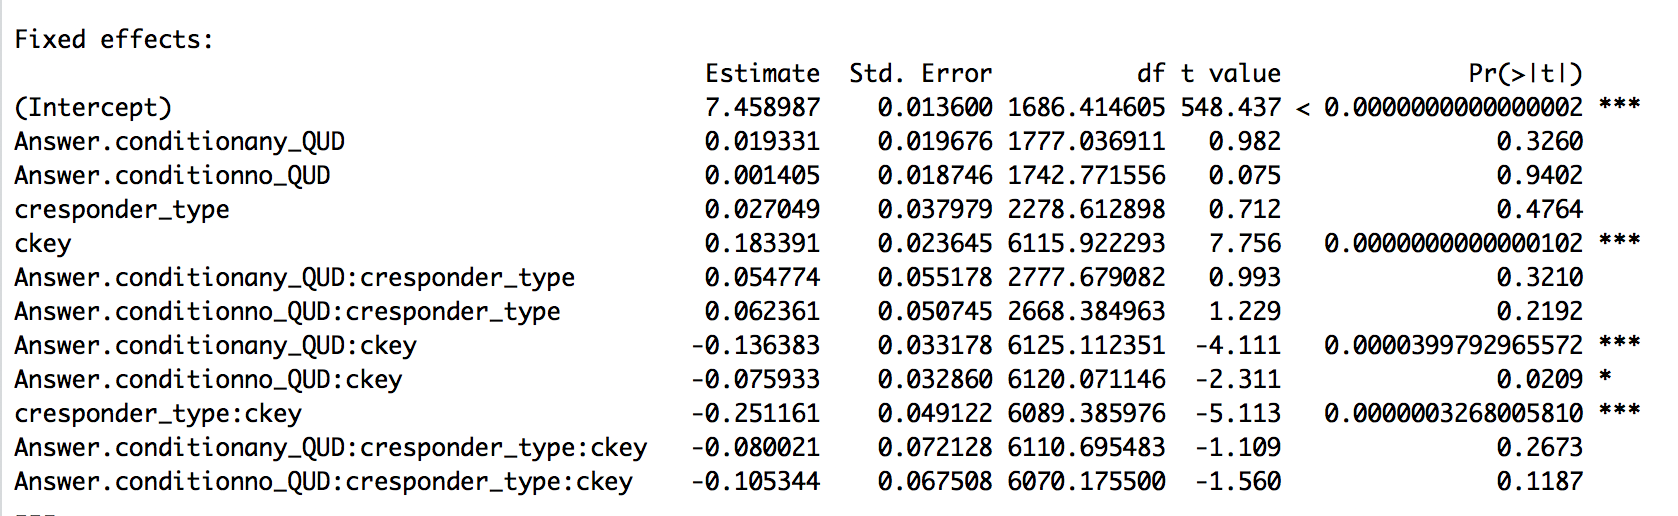
\includegraphics[height=10cm]{models/exp4_model3.pdf}
\pagebreak
\item Mixed effects linear regression model with random by-participant intercepts predicting log-transformed response time from fixed effects of QUD, response type, responder type and their interaction
\\
\textbf{Prediction:} Prediction
% \caption*{Model4}
% \includegraphics[height=10cm]{models/exp4_model4.pdf}
\end{enumerate}
\pagebreak

\section*{Models - for experiment 3 (age groups)}
\begin{enumerate}    
\item Mixed effects logistic regression predicting response type with random by-participant intercepts, from fixed effects of QUD, age and their interaction
\\
\textbf{Prediction:} Interaction of QUD and age such that in the younger age group(18-25) there are more pragmatic responses for all-QUD compared to any-QUD and no-QUD
\\ \\
% \caption*{Model1}
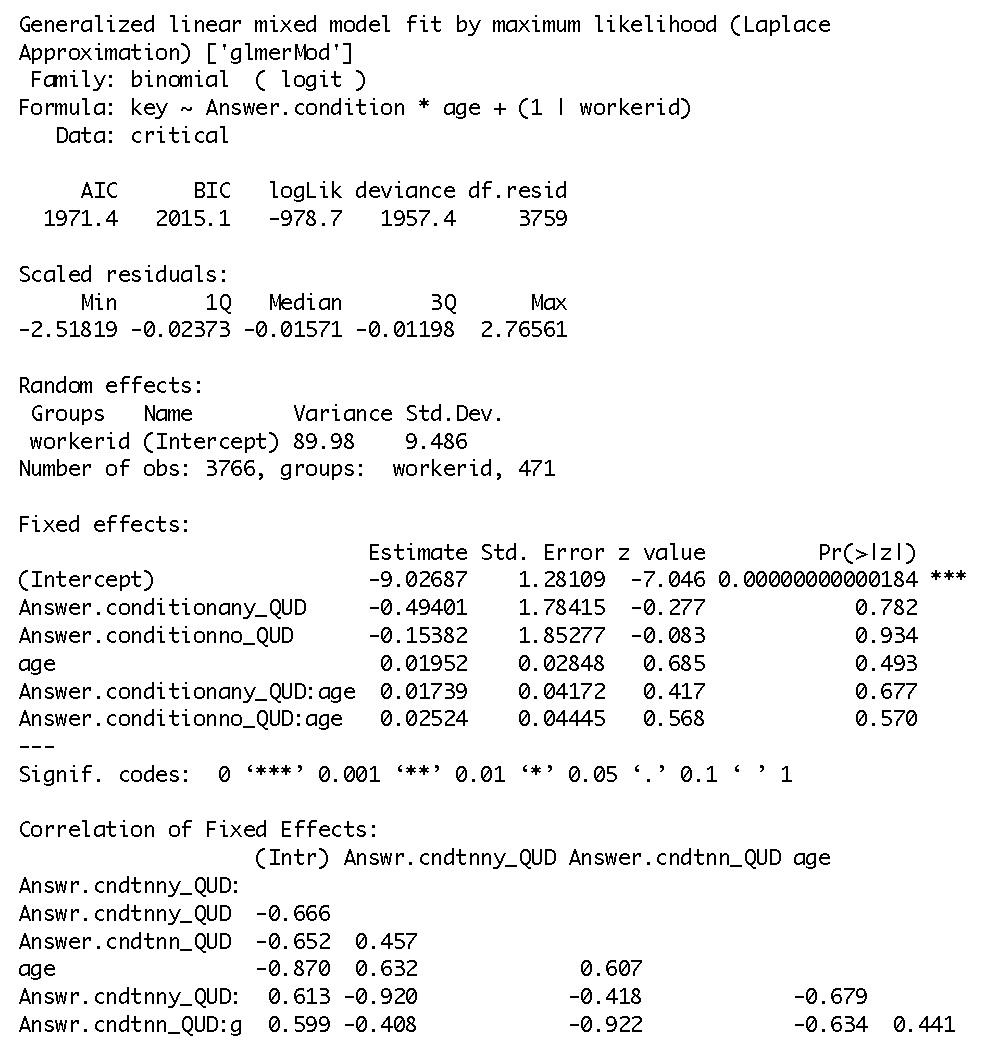
\includegraphics[height=10cm]{models/exp3_model1.pdf}
\pagebreak
\item Mixed effects linear regression model with random by-participant intercepts predicting log-transformed response time from fixed effects of QUD, response type, age and their interaction
\\
\textbf{Prediction:} Interaction of QUD, response and age such that in the younger age group(18-25) the more relevant the alternative, the faster the pragmatic responses become and the slower the semantic responses become.
\\ \\
% \caption*{Model2}
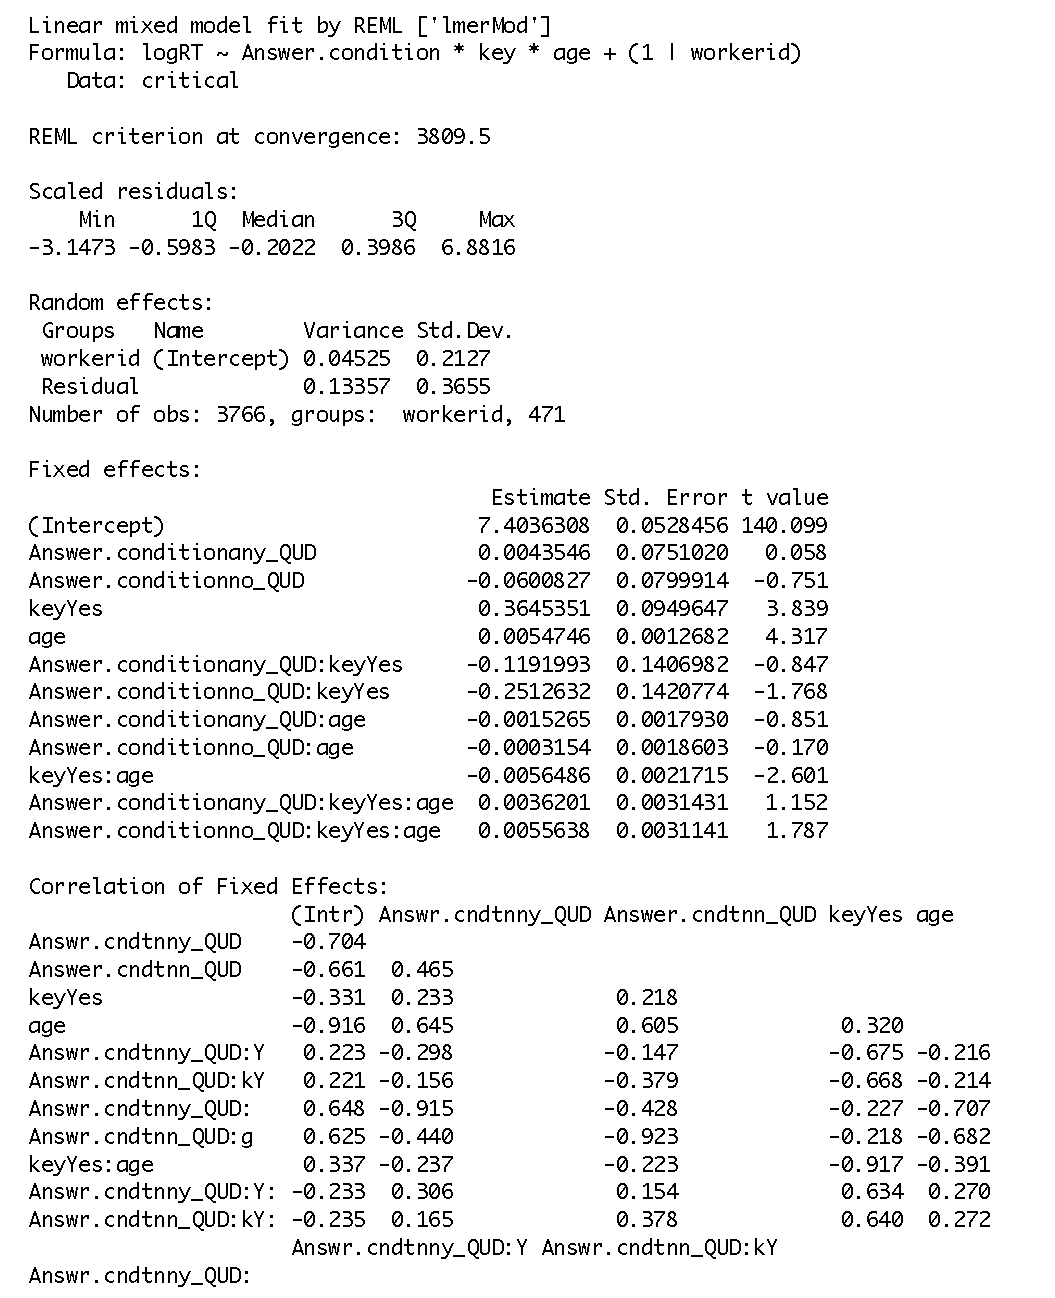
\includegraphics[height=10cm]{models/exp3_model2_1.pdf} \\
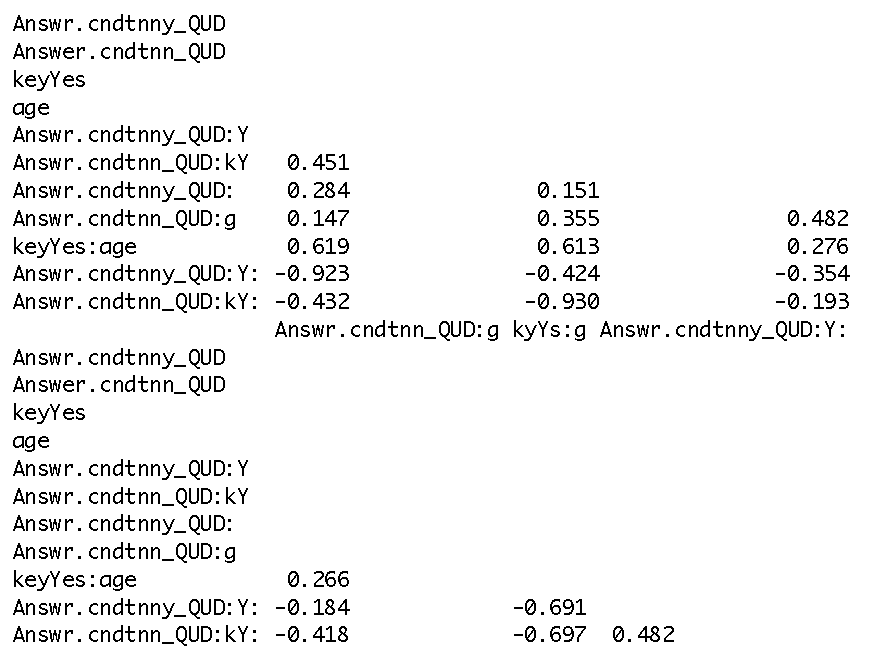
\includegraphics[height=6cm]{models/exp3_model2_2.pdf}
\end{enumerate}


\pagebreak
% \section*{Formatting Citations}
\bibliography{scibib}
\bibliographystyle{Science}
\end{document}




















